\chapter{Design Approach} \label{chap:designaproach}
%%%%%%Intoduction/description
Based on the requirements mentioned in Section \ref{sec:requirements} the approach shown in \autoref{fig:controllerDiagram} can be designed to autonomously survey an area specified by four X-Y points.
\begin{figure}[H]
    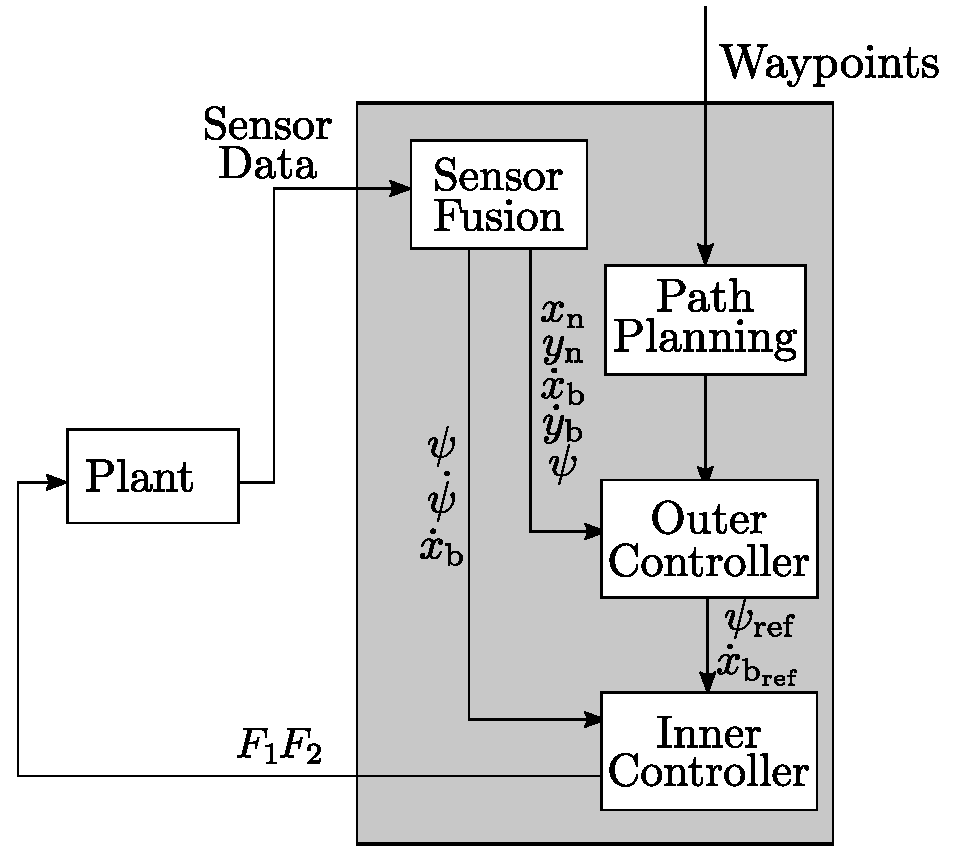
\includegraphics[width=0.3\textwidth]{figures/controllerDiagram2}
    \caption{Diagram of the control approach.}
    \label{fig:controllerDiagram}
\end{figure}
This is achieved by computing a path within the specified area, that preforms a sweeping motion with a predefined width. The path is used as input into the controllers, making the vessel follow it. 

%%%%% Path generation
The control design consists of two controllers, an inner controller and an outer controller. 

As shown on \autoref{fig:controllerDiagram} the outer controller is in charge of following the path by changing the reference of the inner controller to obtain its desired position. Using $x_\mathrm{n}$ , $y_\mathrm{n}$ $x_\mathrm{b}$ $y_b$ and $\psi$ it is able to compute the $\psi_\mathrm{ref}$ and $x_\mathrm{ref}$ needed to follow the path. 

The inner controller uses this references to control $\dot{x}_\mathrm{b}$ and $\dot{\psi}$ by asking for the appropriate $F_{1}$ and $F_{2}$ commands. Two design approaches are tested for the inner controller, an $H_{\infty}$ Controller and a Linear Quadratic Regulator.

The $H_{\infty}$ Controller is designed to be robust towards wind and wave disturbances and towards model errors. The LQR controller, on the other side, is designed to reduce the energy consumption of the vessel as well as to drive the states to the reference values as fast as possible. 
The two approaches for the inner controller are then tested in simulation, to compare the robustness and performance of both of them. \fxnote{Make sure this is correct}

%%%%%Sensor Fusion%%%%%%
Additionally, to improve the precision of the measurements, the sensor data is fused together before it is used as input for the controllers. Two Kalman filters, one for the attitude and another one for the translational behavior are used to filter the measurements, which are based on the model of the vessel. 
 
The filter fuses then the measured sensor data into $\psi$, $x_{b}$, $y_{b}$, $\dot{x}_{b}$ and $\dot{y}_{b}$ which are the states used by the controllers. 

In \autoref{chap:innercontrol} the inner controller design is included while the outer control is described in \autoref{chap:outerController}. The sensor fusion is then presented in \autoref{chap:sensorFusion}.

